\documentclass{article}
\usepackage[utf8]{inputenc}
\usepackage[margin=0.75in]{geometry}

\usepackage{enumitem}
\usepackage{siunitx}
\usepackage{graphicx}

\setlength{\parskip}{1em}

\begin{document}
    \begin{center}
        
		\LARGE{\textbf{Proposal Tugas Akhir}} \\
        \vspace{1em}
        \Large{\textit{PM for PM2.5}: Analisis pada Dataset \textit{Air Quality}} \\
        \vspace{1em}
        \normalsize\textbf{Andrew Savero Ongko, Muhammad Fakhrillah Abdul Azis,} \\
        \normalsize\textbf{Muhammad Yudistira Hanifmuti} \\
        \normalsize{\{andrew.savero, muhammad.fakhrillah, muhammad.yudistira\}@ui.ac.id} \\
        \vspace{1em}
        \normalsize{Universitas Indonesia, Depok} \\
        \normalsize{Fakultas Ilmu Komputer}

	\end{center}
    \begin{normalsize}
        
        \section{Identifikasi Masalah}
        Proposal ini dimulai dengan identifikasi dari masalah yang ingin diselesaikan. 
        Pada kesempatan ini, kelompok kami mendapatkan dataset \textit{Air Quality} 
        untuk pengerjaan Tugas Akhir Mata Kuliah Penambangan Data. Dataset tersebut memiliki 
        sebuah atribut target bernama "PM 2.5" dan beberapa atribut lain yang merupakan hasil 
        pengawasan kualitas udara oleh beberapa stasiun pengawasan di suatu negara. Atribut 
        PM2.5 merujuk pada istilah \textit{"Atmospheric Particulate Matter"} yang memiliki
        diameter $<$ \SI{2.5}{\micro\metre}. Ukurannya yang kecil membuat partikel ini dapat 
        masuk jauh ke dalam sistem pernafasan dan peredaran darah yang dapat menyebabkan 
        serangan jantung, penyakit pernafasan, hingga kematian. Sehingga konsentrasi PM2.5
        ini cukup penting untuk dimonitor dan diproses lebih lanjut. Hal ini dapat membantu 
        mengetahui tempat dan waktu krusial yang memiliki tingkat PM2.5 tinggi agar bisa
        dilakukan usaha pencegahan untuk menghindari hal-hal yang tidak diinginkan.

        \noindent Seperti yang disinggung pada paragraf sebelumnya, dataset \textit{Air Quality}
        berisikan atribut yang menjelaskan kondisi kualitas udara, seperti suhu dan tekanan udara,
        pada suatu waktu di suatu tempat tertentu. Pada setiap baris pada dataset, terdapat kolom
        PM2.5 yang menyatakan konsentrasi partikel PM2.5 yang ada di udara dalam satuan 
        (ug/\SI{}{\metre\cubed}). Kami akan mencoba membuat model \textit{machine learning} yang 
        dapat mempelajari pola kualitas udara agar bisa digunakan untuk memprediksi kadar PM2.5 
        di udara. Metode \textit{data mining} yang digunakan adalah \textit{Regression} karena 
        nilai kadar PM2.5 yang menjadi target bersifat kontinu (ug/\SI{}{\metre\cubed}). Oleh
        karena itu, kami akan menerapkan metode dan langkah-langkah yang biasa digu=nakan untuk
        membangun model \textit{Regression}.

        \section{Hasil Eksplorasi Data}
        Bagian ini menjelaskan hasil eksplorasi data yang telah kami lakukan dalam mengolah 
        dataset \textit{Air Quality}. Hasil yang disampaikan juga dilengkapi dengan beberapa
        asumsi yang kami gunakan selama mengolah data.
        
        \subsection{\textit{Dirty Data} dan \textit{NaN Values}}
        Pada dataset, kami menemukan beberapa baris data yang merupakan duplikasi dari \textit{header}
        seperti yang dapat dilihat pada baris 1794 pada Figure 1. Untuk setiap baris tersebut kami buang
        dari dataset karena tidak relevan.

        \begin{figure}[h!]
            \centering
            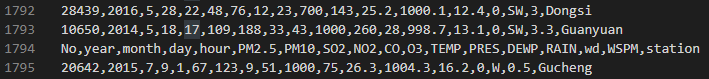
\includegraphics[width=0.8\linewidth]{dirty_data.PNG}
            \caption{Duplikasi \textit{header}.}
            \label{fig:dirty_data}
        \end{figure}

        \noindent Selain duplikasi \textit{header}, kami juga menemukan beberapa baris data yang memiliki nilai NaN
        pada sebagian kolomnya. Untuk masalah ini, kami mengasumsikan bahwa baris data tersebut sebaiknya
        dibuang terlebih dahulu. Namun, terdapat kemungkinan untuk diberikan penanganan pada nilai NaN 
        tersebut pada tahap selanjutnya.

        \subsection{\textit{Data Summary}}
        Kami sudah membuat beberapa \textit{summary} dari data, terutama untuk atribut numerik selain target yang
        dapat dilihat pada Figure 2. Dari persebaran yang ditunjukkan pada Figure 2, kami menduga bahwa beberapa 
        atribut memiliki nilai yang merupakan \textit{outlier}. Oleh karena itu, butuh diolah lebih lanjut sebelum
        nantinya data latih tersebut akan digunakan untuk melatih model \textit{machine learning}.
        \begin{figure}[h!]
            \centering
            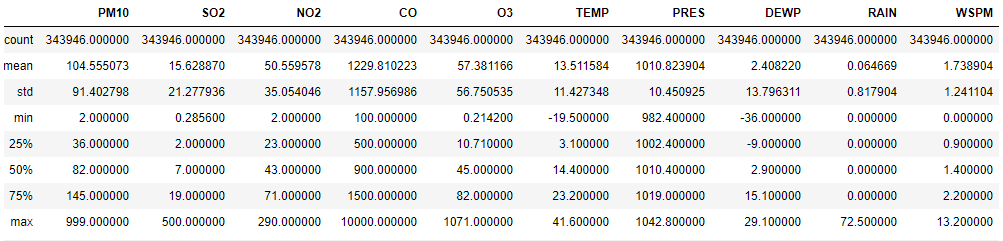
\includegraphics[width=\linewidth]{data_summary.PNG}
            \caption{\textit{Data Summary}}
            \label{fig:data_summary}
        \end{figure}

        \subsection{\textit{Correlation Matrix}}
        Hal lain yang perlu diperhatikan dari data tabular seperti dataset ini adalah matriks korelasinya. Dengan
        mengetahui korelasi antar atribut, atribut yang redundan dapat dikenali sehingga dapat ditentukan untuk 
        dibuang sebagian atau tidak. Di bawah ini adalah Figure 3 yaitu matriks korelasi dari dataset \textit{Air Quality}.
        \begin{figure}[h!]
            \centering
            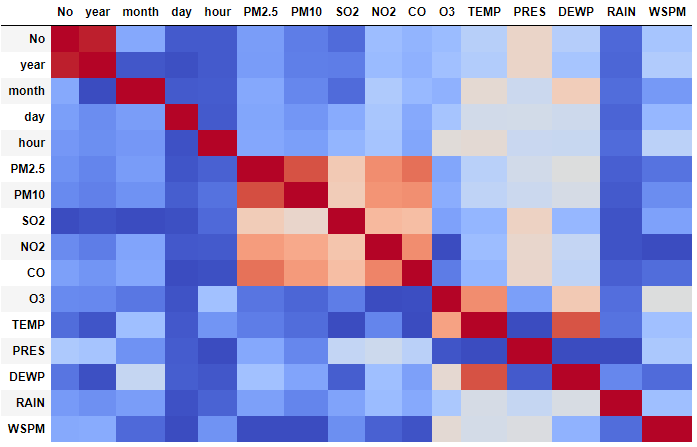
\includegraphics[width=0.5\linewidth]{corr_mat.PNG}
            \caption{\textit{Correlation Matrix}}
            \label{fig:corr_mat}
        \end{figure}
        Warna merah pada Figure 3 menunjukkan korelasi positif dan warna biru menunjukkan adanya korelasi negatif.
        Semakin gelap warna pada matriks menunjukkan hubungan korelasi yang lebih kuat. Dapat dilihat bahwa beberapa
        atribut memiliki korelasi yang lebih kuat terhadap PM2.5, seperti PM10, CO dan RAIN. Hal ini dapat menjadi
        pertimbangan untuk memilih kolom-kolom yang lebih relevan terhadap prediksi nanti.

        \section{Desain Cara Kerja}
        Bagian ini menjelaskan desain cara kerja yang dilakukan oleh kelompok kami untuk mengolah dataset yang 
        diberikan. Terdapat beberapa tahapan yang dilakukan saat mengolah data, baik itu yang sudah dilakukan 
        sampai tahap pertama ini, atau yang akan dilakukan nanti pada tahap selanjutnya.

        \subsection{\textit{Data Cleansing Process}}
        \textit{Data Cleansing} adalah langkah pertama yang krusial dalam proses mempersiapkan data secara 
        umum dan juga proses menganalisa, mengidentifikasi dan memperbaiki data yang masih berantakan. Hal ini
        sudah dilakukan pada tahap eksplorasi yang dijelaskan di atas. Beberapa hal yang dilakukan adalah
        sebagai berikut.
        \begin{enumerate}[label=\alph*.]
            \item Menghapus kolom yang tidak terpakai.
            \item Menghapus duplikasi pada baris (namun dapat dibutuhkan pada kasus tertentu).
            \item Menghapus nilai yang datanya belum disimpan atau informasi yang hilang.
            \item Mengubah format data menjadi format yang lebih mudah untuk digunakan.
        \end{enumerate}

        \subsection{Identifikasi Keterkaitan antar Atribut atau Fitur}
        Tujuan utama dari identifikasi ini adalah mengenali dan membuat hubungan kerterkaitan yang dapat
        mendukung pembuatan hipotesis. Hal ini dapat dilakukan dengan membuat matriks-matriks keterhubungan,
        seperti matriks korelasi dan matriks kovarian.

        \subsection{\textit{Preprocessing}}
        Pada tahap ini, data akan diolah terlebih dahulu supaya dapat distandarisasi. Proses ini harus dilakukan
        sebelum model \textit{machine learning} dilatih dan saat membuat prediksi. Bagian ini belum dijelaskan
        secara mendalam karena kami belum sampai pada tahap ini, begitu pula tahap yang akan dijelaskan selanjutnya.

        \subsection{\textit{Candidate Models Generation}}
        Di sini merupakan tahap utama dari penggunaan algoritma yang sudah dipelajari di kelas Penambangan Data.
        Model yang akan dibuat tidak hanya satu jenis saja, namun dibuat sebanyak mungkin sehingga performa dari
        setiap model dapat dibandingkan dan didapatkan model terbaik. Metode yang digunakan akan dijelaskan pada
        poin selanjutnya (poin 4).

        \subsection{Evaluasi Model}
        Tujuan dari evaluasi model adalah memahami dengan baik performa dari setiap model yang sudah dibuat.
        Evaluasi dilakukan dengan menghitung beberapa jenis nilai metrik yang umum digunakan untuk mengevaluasi
        model. Nilai-Nilai tersebut kemudian akan digunakan sebagai pertimbangan untuk memperbaiki model yang
        sudah dibuat.

        \section{Metode yang Digunakan}

        Pada paragraf pembuka di atas, kami sudah menyatakan bahwa masalah ini dapat diselesaikan dengan menggunakan
        metode \textit{Regression}. Kami bermaksud untuk menggunakan beberapa jenis algoritma regresi, seperti
        \textit{linear regression}, \textit{decision tree reggressor} dan algoritma lainnya. Semua algoritma 
        tersebut akan dibandingkan atau dikolaborasikan dengan konsep \textit{boosting, bagging} dan 
        \textit{stacking} seperti yang sudah dijelaskan di kelas. Tujuan dari pendekatan tersebut adalah ketidakmampuan
        model sederhana untuk memahami sebuah masalah atau dataset yang rumit (terkait linearitas). Pendekatan 
        menggunakan beberapa model juga sudah menjadi hal yang umum dalam Penambangan Data sampai hari ini.
        Penjelasan terkait istilah di atas akan dijelaskan sebagai berikut.

        \subsection{\textit{Bagging}}

        \textit{Bagging} adalah singkatan dari \textit{Bootstrapping and Aggregating}. \textit{Bootstrapping} adalah 
        sebuah metode untuk mengurangi varians dari sebuah model dan mengurangi \textit{overfitting}, dengan melakukan
        \textit{sampling} ulang data dari data latih dengan kardinalitas yang sama dengan data awal sehingga tercipta
        sejumlah sampel. Model yang terbuat adalah sejumlah dengan sampel sehingga hasilnya diharapkan tidak begitu 
        \textit{overfit} dibandingkan dengan model tunggal.

        \subsection{\textit{Boosting}}

        Ide utama dari \textit{Boosting} adalah menyusun beberapa model secara sekuensial. Dengan setiap iterasi 
        \textit{boosting}, model baru akan dibuat dengan model tersebut dilatih berdasarkan error-error yang terjadi
        pada model sebelumnya.

        \subsection{Stacking}

        \textit{Stacking} adalah bentuk model ensemble lain, yaitu sebuah model baru dilatih menggunakan gabungan prediksi
        dari 2 model sebelumnya atau lebih. Prediksi dari model-model tersebut digunakan sebagai \textit{input} untuk 
        setiap \textit{sequential layer}, dan dikombinasikan menjadi sebuah set prediksi yang baru. Set prediksi baru ini 
        dapat dipakai pada layer tambahan lagi, atau cukup berhenti di situ sebagai hasil akhir.

        \section{Referensi}

        Referensi yang digunakan selama penyusunan proposal ini.
        \begin{itemize}
            \item https://towardsdatascience.com/hitchhikers-guide-to-exploratory-data-analysis-6e8d896d3f7e
            \item https://medium.com/@rrfd/boosting-bagging-and-stacking-ensemble-methods-with-sklearn-and-mlens-a455c0c982de
        \end{itemize}
    \end{normalsize}
  
\end{document}